\documentclass[a4paper]{scrreprt}

%% Language and font encodings
\usepackage[english]{babel}
\usepackage[utf8x]{inputenc}
\usepackage[T1]{fontenc}

%% Sets page size and margins
\usepackage[a4paper,top=3cm,bottom=2cm,left=3cm,right=3cm,marginparwidth=1.75cm]{geometry}

%% Useful packages
\usepackage{amsmath}
\usepackage{graphicx}
\graphicspath{ {./img/} }
\usepackage[colorinlistoftodos]{todonotes}
\usepackage[colorlinks=true, allcolors=blue]{hyperref}

\title{Hattori}
\subtitle{"A vertical-scrolling space-shooter"}
\author{Edward Eldridge (G00337490)}
\titlehead{\centering
\includegraphics[width=15cm]{HattoriLogo}}


\begin{document}
\maketitle

\begin{abstract}

 Hattori will attempt to re-invent the traditional vertical scrolling space shooter genre by retaining the core gameplay while introducing more interactivity and decision making with the addition of a resource management system, on-screen gestures and a detailed upgrade system. 

\end{abstract}

{
  \hypersetup{linkcolor=black}
  \tableofcontents
}

% ______________________
% chapter Overview
% ______________________
\chapter{Overview}

Traditionally, a vertical scrolling space shooter consists of the player controlling a spaceship while 'aliens' or enemies attempt to destroy the players ship.
While this kind of gameplay can be fun, for me personally it quickly loses it's charm as aside from controlling the ship and shooting, there is little else for the player to do. With Hattori, I intend to add an extra layer of depth to the core gameplay of this genre.



\begin{enumerate}
  \item \textbf{Resource management}
  \begin{itemize}
    \item Link the player's score with the use of special abilities.
    \item Introduces risk/reward. The player must decide if it is necessary to use a special ability. Overuse of abilites will result in a lower score but not enough use could result in the player losing. Player must find a balance.
  \end{itemize}
  \item \textbf{Gesture-based combat}
  \begin{itemize}
    \item Rather than the traditional method of defeating enemies through just moving and firing, I intend to introduce abilities that require on-screen gestures to be performed. For example, drawing a circle could represent a bomb, or a cross a sword strike.
    \item This addition will provide more depth to the game and give the player an opportunity to interact more with the game. Maybe the player is poor at managing his energy/score but can quickly perform gestures. giving them an advantage vs. other players.
  \end{itemize}
  \item \textbf{Player upgrade}
  \begin{itemize}
    \item To keep players interested, I intend to introduce a way of augmenting or upgrading the player's ship.
    \item Upgrade systems and character development are very important aspects to any game. They provide the player with a feeling of accomplishment and progress. They also keep the game fresh and exciting as more ways to play the game are introduced as the player progresses through the game.
  \end{itemize}

\end{enumerate}

% ______________________
% chapter References
% ______________________

\chapter{References} 
\href{https://www.gamasutra.com/view/feature/130452/improving_player_choices.php}{Improving Player Choices by Tracy Fullerton, Chris Swain and Steve Hoffman}
% ______________________
% chapter Specification and Market Analysis 
% ______________________

\chapter{Specification}

\section{Genre}
Hattori will be a score-based, endless, vertical-scrolling shooter.

\begin{figure}[h]
  \centering
  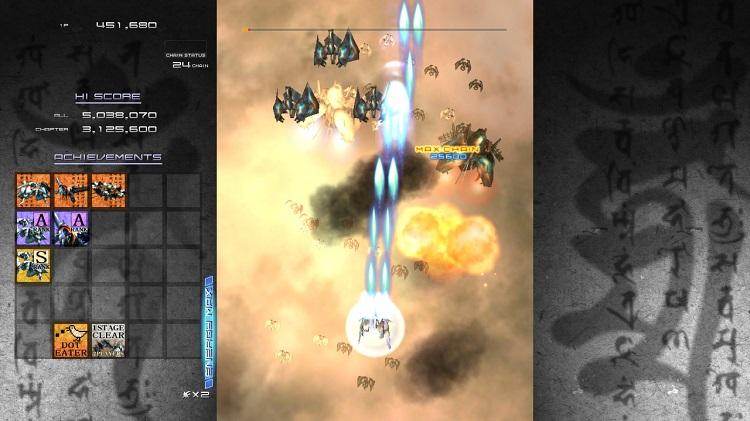
\includegraphics[width=0.7\textwidth]{IkaguraGameplay}
  \caption{\label{fig:art}Gameplay from Ikagura(1998)}
  \end{figure}

  \begin{figure}[h]
    \centering
    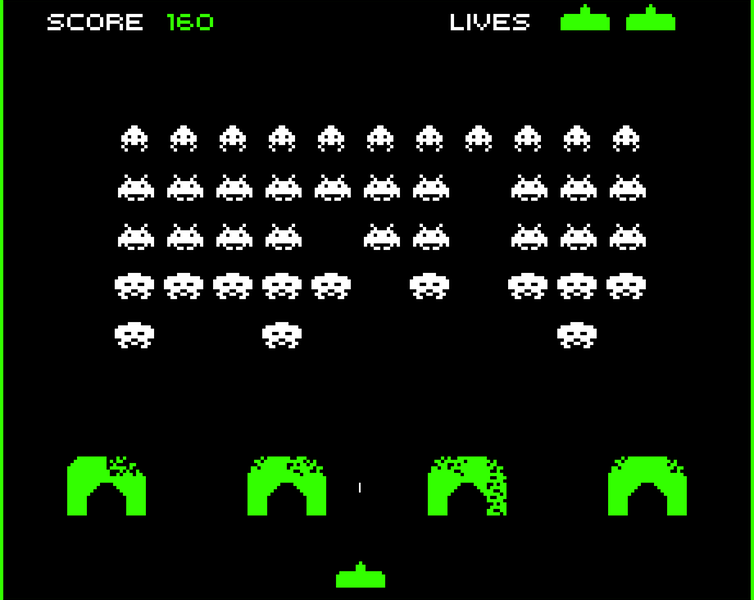
\includegraphics[width=0.7\textwidth]{Invaders}
    \caption{\label{fig:art}Gameplay from Space Invaders(1978)}
    \end{figure}

\clearpage

\section{Art Style}
The art style of the game will be mainly sci-fi/space focused but will take inspiration from lots of different sources. 

\begin{figure}[h]
  \centering
  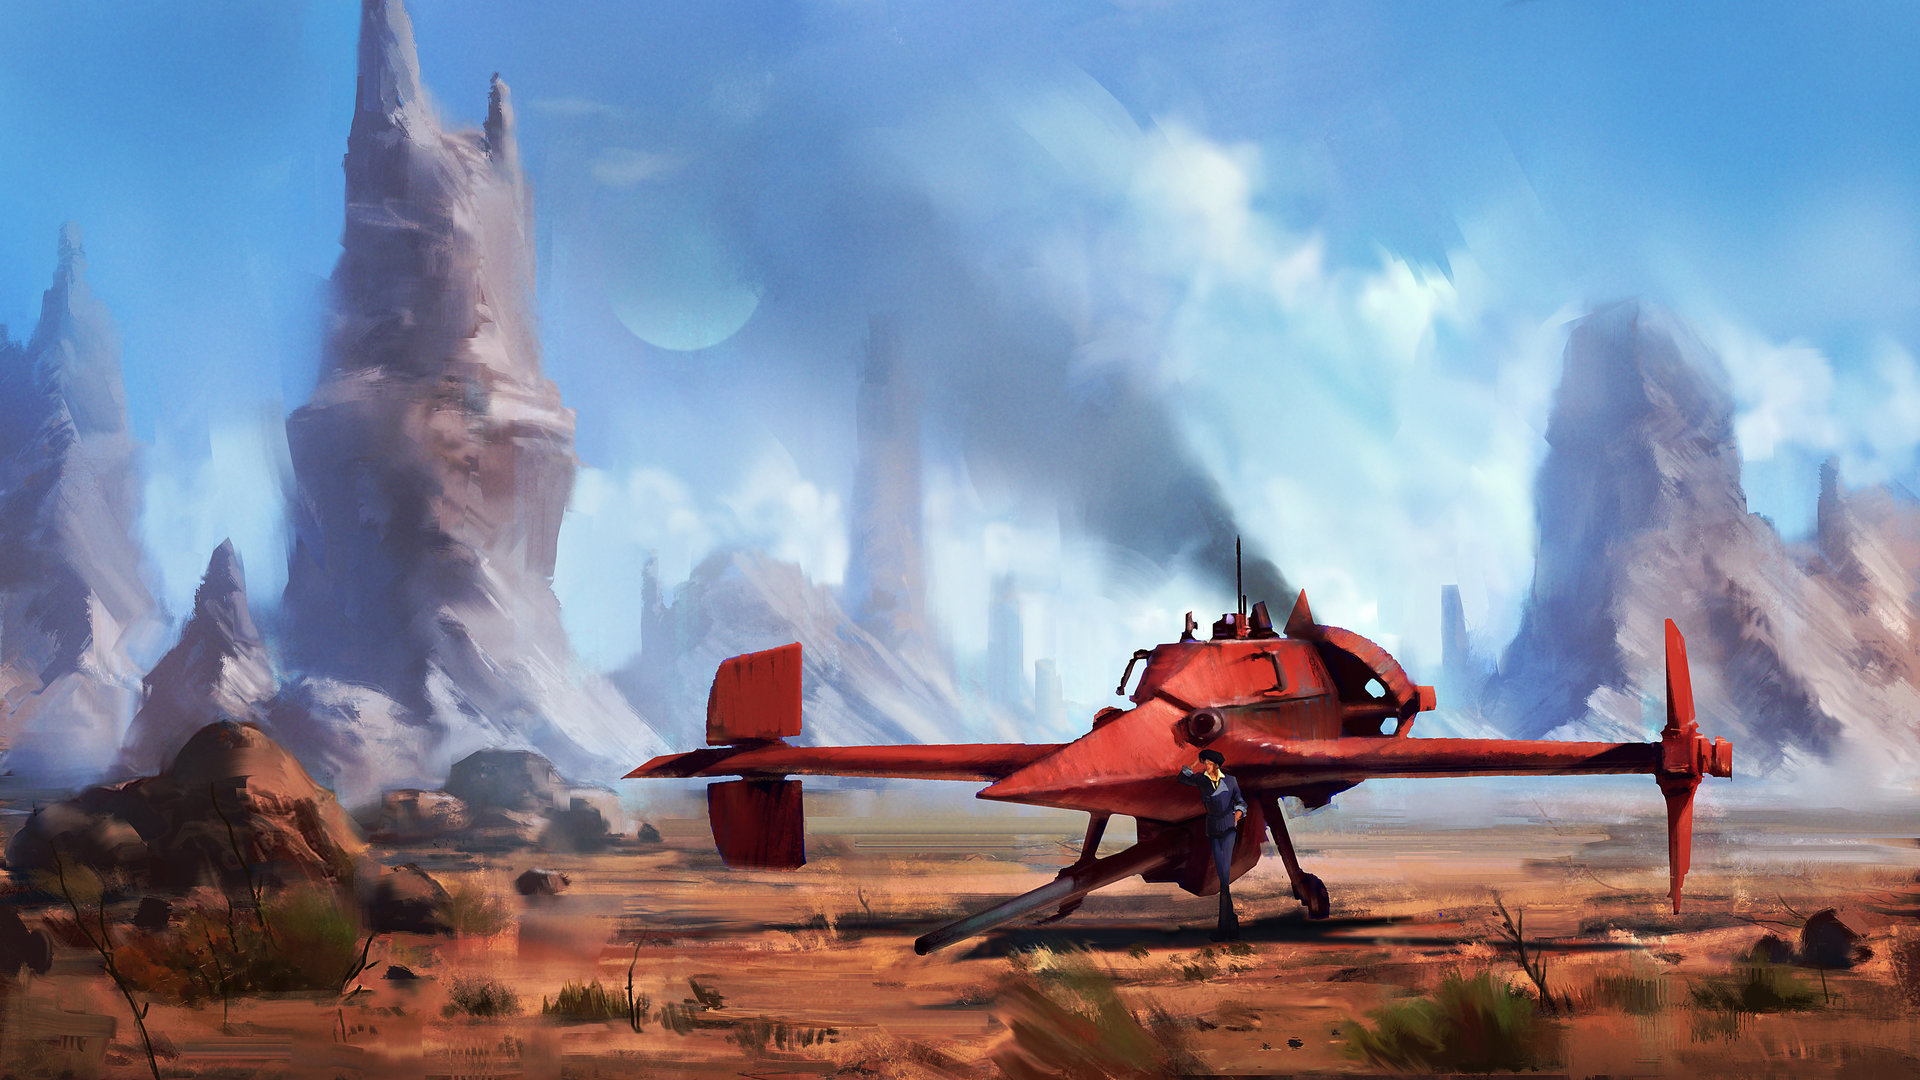
\includegraphics[width=0.8\textwidth]{Spaceship}
  \caption{'Cowboy Bebop' concept art}
  \end{figure}

  \begin{figure}[h]
    \centering
    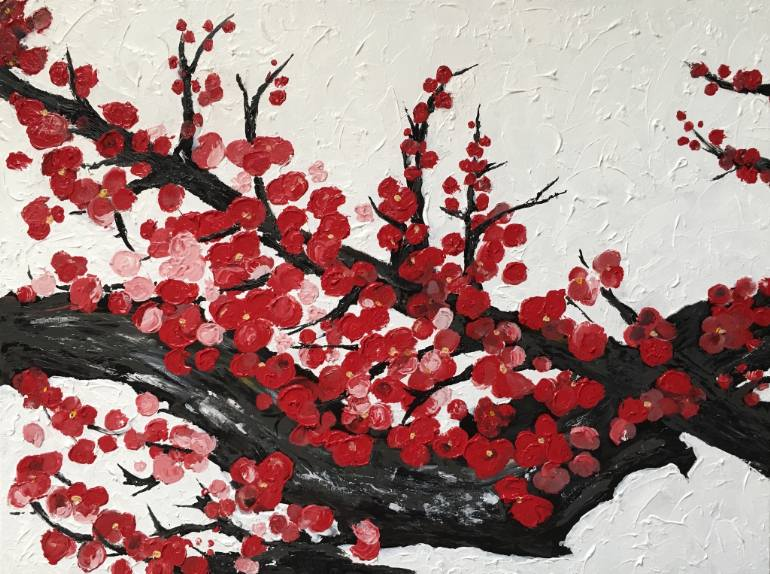
\includegraphics[width=0.8\textwidth]{cherry}
    \caption{Cherry blossom painting}
    \end{figure}
\chapter{Gameplay and Game Setting}
\section{Story}
The story of the game will be kept simple to instead focus on gameplay. While exploring space in a ship called the 'Hattori', the player is teleported to an unknown location in space. The player is then confronted by horde of enemies they must defeat to survive.

\section{World/Environment}
The game will be set in space. As such, the background and enviroment may feel a bit bland, however due to the nature of the story I can expand on this and hope to make the player feel like they are making some kind of progress through space instead of feeling like a static object on a scrolling background. 

\begin{figure}[h!]
  \centering
  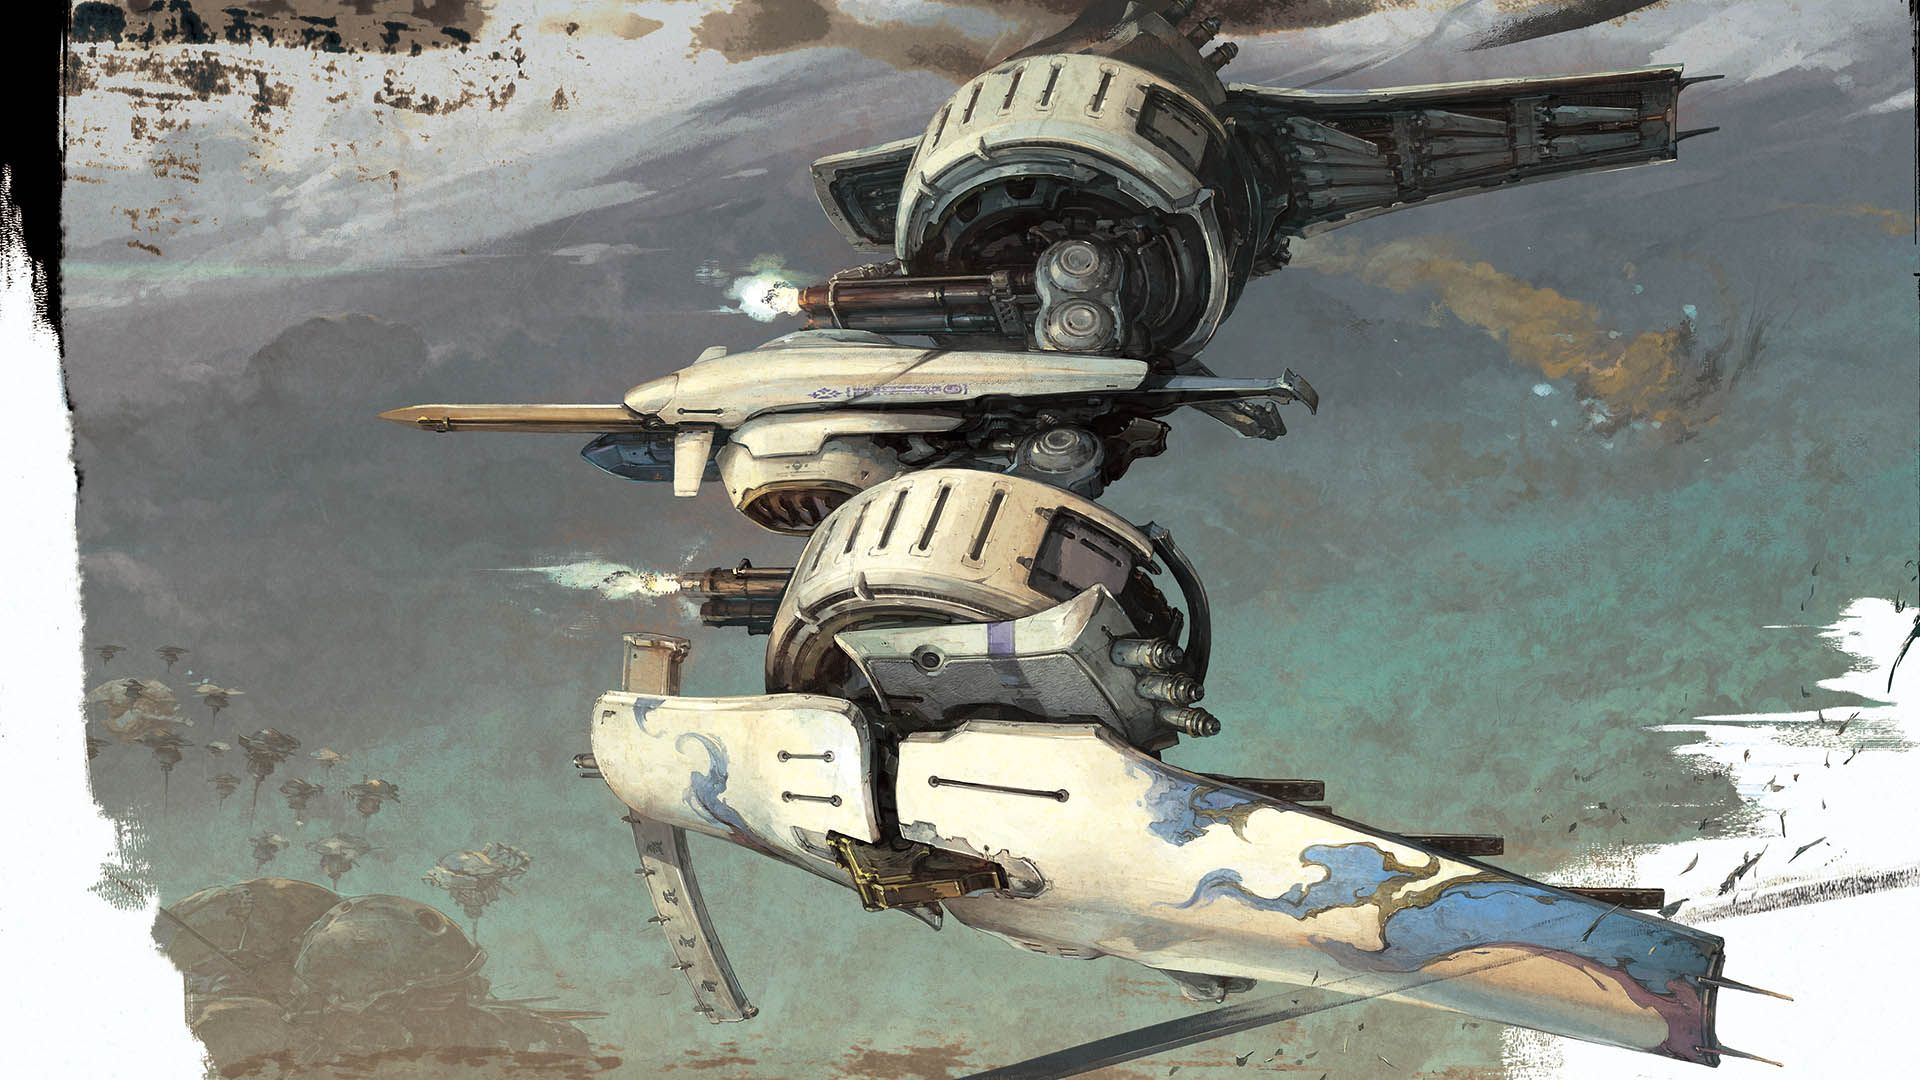
\includegraphics[width=1\textwidth]{Ikagura}
  \caption{\label{fig:art}Art from Ikagura(1998)}
  \end{figure}

\clearpage

\section{User Interface}
The user interface of the game will be broken down into 3 sections. 
\begin{itemize}
  \item A large health bar so the player will be able to know their current health without moving their eyes away from the action. 
  \item The general gameplay area, where the player will be controlling the ship and where enemies will be spawning. 
  \item A third area for additional information such as the player's score, upgrades, special abilities etc.
\end{itemize}

\begin{figure}[h]
  \centering
  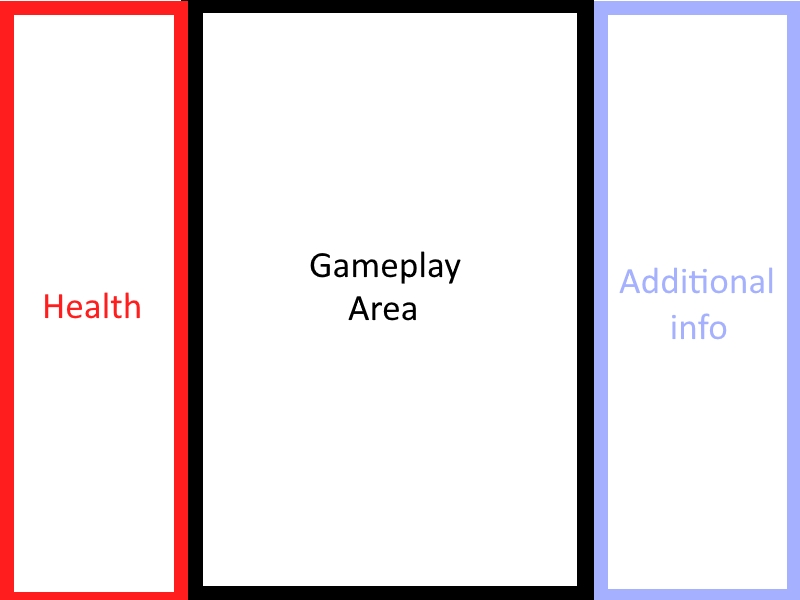
\includegraphics[width=1\textwidth]{UI}
  \caption{\label{fig:art}UI Example}
  \end{figure}

\section{Main Objective}
The main objective of the game is to stay alive. At the end of each round/wave, the player will have a chance to rest and take count of his resources, health and current upgrades.
This will give the player a break to either stop/playing continue. This allows the player to not feel like playing a round is a time commitment and makes the game generally more accessible to a wider audience.

\clearpage

\section{Core Mechanics}
ttt
\begin{figure}[h!]
  \centering
  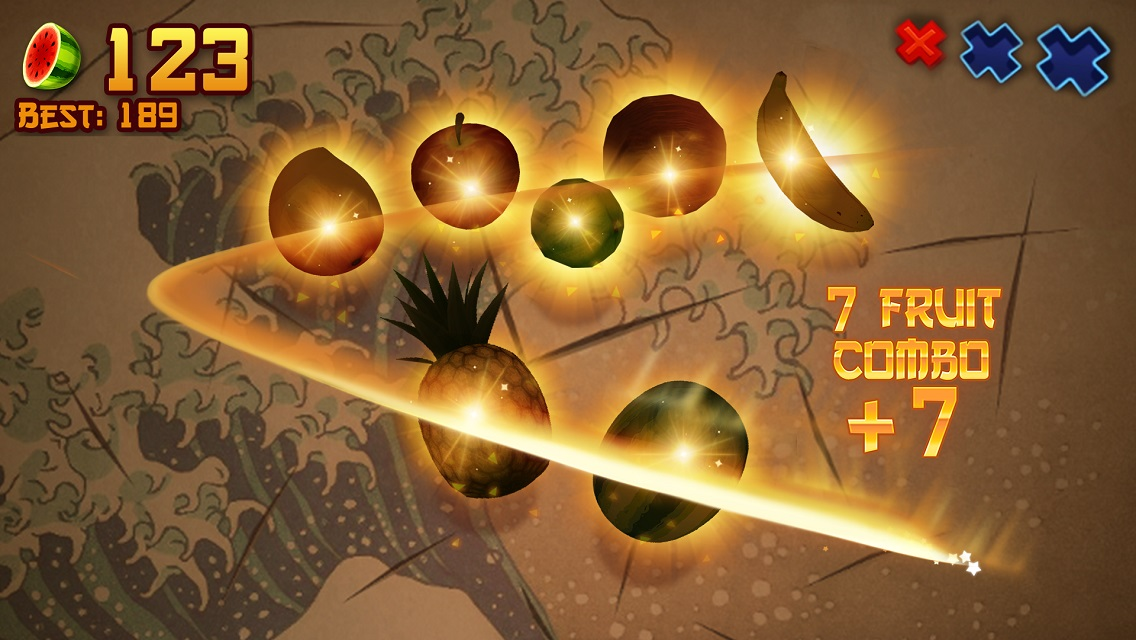
\includegraphics[width=1\textwidth]{FruitNinja}
  \caption{Gameplay from 'Fruit Ninja'(2010)}
  \end{figure}

\section{Controls}
describe the controls of the game 
also, add here a controller diagram if necessary 

% ______________________
% chapter Front End
% ______________________


\chapter{Front End}
description of front end such as start screen, menu screens,..  

\section{Start Screen}

\section{Menus}

\section{End Screen}

% ______________________
% chapter Game Details
% ______________________


\chapter{Technology}
This game is designed for the Universal Windows Platform but will hopefully be available in both desktop and mobile versions.

\section{Target Systems}
Android, Windows desktop and Universal Windows Platform.

\section{Hardware}
Mouse and keyboard or an accelerometer/touch screen device.

\section{Development Systems/Tools}
\begin{enumerate}
  \item \textbf{Programming}
  \begin{itemize}
    \item The game will be developed in the \textbf{Unity} engine, using the Unity editor. 
    \item \textbf{C\#} wil be the main programming language, using \textbf{Visual Studio 2017/Visual Studio Code} as an IDE.
  \end{itemize}
  \item \textbf{Design}
  \begin{itemize}
    \item \textbf{Paint.net} will be used to to design the art/assets.
    \item \textbf{Audacity} and royalty-free music/sound effects will be used to create the audio component.
  \end{itemize}
  \item \textbf{Source control/Documentation}
  \begin{itemize}
    \item \textbf{Git} and \textbf{GitHub} are the technologies being utilized for source control. 
    \item This design document and documentation will be created with a combination of \textbf{LaTeX} and \textbf{Markdown}.
  \end{itemize}

\end{enumerate}


  
% ______________________
% chapter Game Details
% ______________________



\chapter{Timeline}
\begin{table}[h]
\centering
\begin{tabular}{|l|l|l|}
\hline
\textbf{Milestone} & \textbf{Description} & \textbf{Date} \\\hline
& Official Start Date & 12.09.2018 \\
1 & Basic gameplay mechanics  & 31.09.2018 \\
2 & Upgrade/resource system  & 14.10.2018 \\
3 & User interface/menus &31.10.2018 \\
4 & Music/SFX & 7.11.2018 \\
5 & Bugfixing & 21.11.2018 \\
5 & Documentation & 24.11.2018 \\
& End of Project & 31.11.2018 \\
\hline
\end{tabular}
\end{table}
% ______________________
% chapter Game Details
% ______________________

\end{document}